\documentclass{article}

% 导入中文宏包
\usepackage{ctex}
\usepackage{array}
\usepackage{caption}
\usepackage{hyperref}
% 设置页面边距
\usepackage{geometry}
\usepackage{graphicx}
\geometry{a4paper, left=2.5cm, right=2.5cm, top=3cm, bottom=3cm}

% 设置标题、作者和日期
\title{元编程和Pytorch编程}
\author{23020007160  张绍延}

\begin{document}

% 生成标题、作者和日期
\maketitle

% 心得报告正文
\section{实验目的}
本次课程主要讲授了代码的调试及性能分析、元编程和Pytorch编程,熟练掌握三者。

\section{介绍}
代码调试和性能分析是确保软件稳定、高效运行的关键步骤。
调试能够帮助开发者在软件出现问题时快速定位并解决问题,
而性能分析则能揭示软件运行时的效率瓶颈,指导开发者进行优化。
这两者共同提高了软件的可靠性和用户体验,
对于维护和改进软件至关重要。

元编程的好处在于它提高了代码的抽象层次和灵活性,
允许程序在运行时自我修改或生成代码。这意味着可以减少重复性代码,
使代码更加简洁,并且能够处理更加复杂和动态的需求。

PyTorch编程的好处则体现在它为深度学习研究者和工程师提供了
一个直观、灵活且高效的工具集。它使得模型构建和调试变得简单,
同时它的社区支持和生态系统为深度学习项目提供了丰富的资源。

\section{练习内容}
\subsection{调试及性能分析学习例子8个}

1.assert的使用
\begin{verbatim}
    def add_positive_numbers(a, b):
       assert a > 0 and b > 0, "Both numbers must be positive"
       return a + b
       # 调试情况,将触发断言错误
       print(add_positive_numbers(-3, 4))
       # 正常情况
       print(add_positive_numbers(3, 4))
\end{verbatim}

 
\noindent
\begin{minipage}{\linewidth}
  \centering
  % 插入图片
  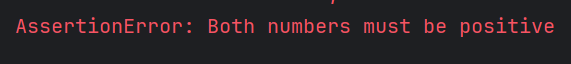
\includegraphics[width=0.5\linewidth]{学习1.png}
  % 图片标题
  \captionof{figure}{assert的使用}
  \label{fig:example}
\end{minipage}


2.pdb断点的使用
\begin{verbatim}
   import pdb
   def add(a, b):
      pdb.set_trace()  # 设置断点
      return a + b
   result = add(3, 4)
   print("Result:", result)
  
   断点操作如下:
   l(或list):列出当前执行点周围的代码。
   n(或next):执行当前行,并停在下一行。
   s(或step):进入函数内部。
   c(或continue):继续执行程序,直到下一个断点。
   q(或quit):退出调试器。
   p(或print):打印表达式的值。
   pp:以更可读的格式打印表达式的值。
   b(或break):设置断点,例如b 10在第十行设置断点。
   clear:清除一个或所有断点。
   a(或args):打印当前函数的参数。
   r(或return):执行函数直到返回。
   j(或jump):跳转到指定行。
   w(或where):打印当前堆栈跟踪。
 \end{verbatim}


\noindent
\begin{minipage}{\linewidth}
  \centering
  % 插入图片
  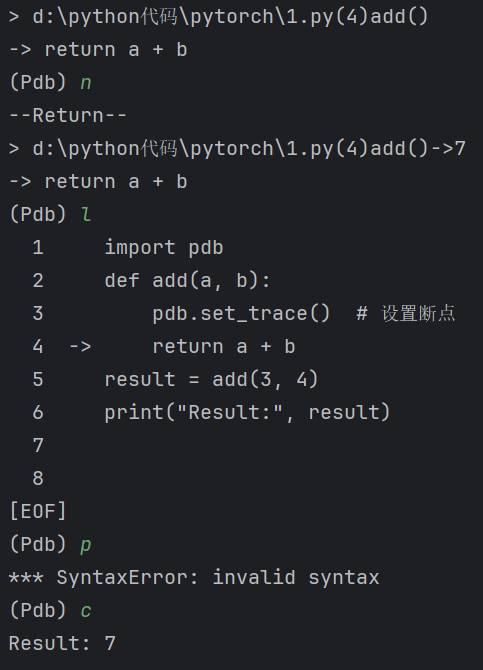
\includegraphics[width=0.5\linewidth]{学习2.png}
  % 图片标题
  \captionof{figure}{pdb断点的设置}
  \label{fig:example}
\end{minipage}

3.使用日志记录调试
 \begin{verbatim}
    import logging
    logging.basicConfig(level=logging.DEBUG)
    def divide(a, b):
       logging.debug(f"Dividing {a} by {b}")
       try:
           result = a / b
       except ZeroDivisionError:
           logging.error("Division by zero!")
           return None
       logging.debug(f"Result is {result}")
       return result
  
    print(divide(10, 2))
    print(divide(10, 0))
 \end{verbatim}

 \begin{verbatim}
   try块中的代码尝试执行除法操作。如果b为0,这将引发ZeroDivisionError异常。这个异常被except块捕
   获,并使用logging.error记录了一条错误信息,表明发生了除以零的错误。最后在运行结束后显示出来。
 \end{verbatim}

\noindent
\begin{minipage}{\linewidth}
  \centering
  % 插入图片
  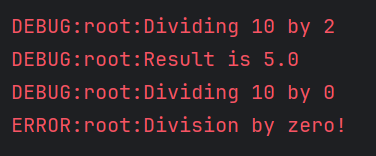
\includegraphics[width=0.5\linewidth]{学习3.png}
  % 图片标题
  \captionof{figure}{日志记录调试}
  \label{fig:example}
\end{minipage}

4.
\begin{verbatim}
   当函数抛出异常时,traceback.print_exc()会打印出异常的堆栈跟踪,帮助定位问题。
    import traceback
    def cause_error():
        return 1 / 0
    try:
        cause_error()
    except Exception:
        traceback.print_exc()
\end{verbatim}

\noindent
\begin{minipage}{\linewidth}
 \centering
  % 插入图片
  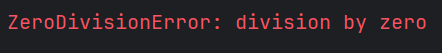
\includegraphics[width=0.5\linewidth]{学习4.png}
  % 图片标题
  \captionof{figure}{traceback模块打印异常信息}
  \label{fig:example}
\end{minipage}



5.
\begin{verbatim}
   这段代码通过cProfile模块记录并分析了example_function的运行时间,
   然后使用pstats模块打印出了性能分析的结果。
    import cProfile
    import pstats
    def example_function():
      total = 0
      for i in range(1000):
          total += i
      return total
    # 使用cProfile运行函数并保存性能数据
    profiler = cProfile.Profile()
    profiler.enable()
    example_function()
    profiler.disable()
    # 打印性能分析结果
    stats = pstats.Stats(profiler).sort_stats('cumtime')
    stats.print_stats()     
\end{verbatim}


\noindent
\begin{minipage}{\linewidth}
 \centering
  % 插入图片
  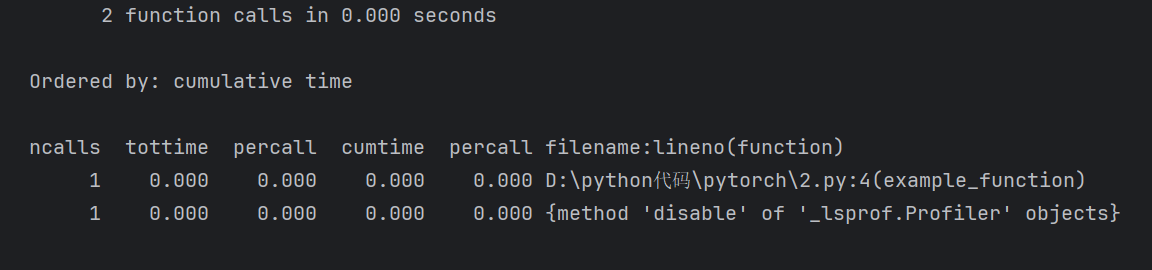
\includegraphics[width=0.5\linewidth]{学习5.png}
  % 图片标题
  \captionof{figure}{cProfile进行性能分析}
  \label{fig:example}
\end{minipage}

6.用timeit重复运行函数并计算平均运行时间
\begin{verbatim}
     import timeit
     import logging
     # 配置日志记录器
    logging.basicConfig(level=logging.DEBUG, format='%(asctime)s - %(levelname)s - %(message)s')
    def debug_example(x):
       logging.debug(f"Entering debug_example with argument: {x}")
       result = x * 2
       logging.debug(f"Exiting debug_example with result: {result}")
       return result
     # 调用函数并观察日志输出
    debug_example(10)
    def performance_test():
       total = 0
       for i in range(1000):
           total += i
       return total
    # 使用timeit重复运行函数并计算平均运行时间
    execution_time = timeit.timeit('performance_test()', globals=globals(), number=1000)
    print(f"Function performance_test executed 1000 times in {execution_time:.4f} seconds")
\end{verbatim}



\noindent
\begin{minipage}{\linewidth}
 \centering
  % 插入图片
  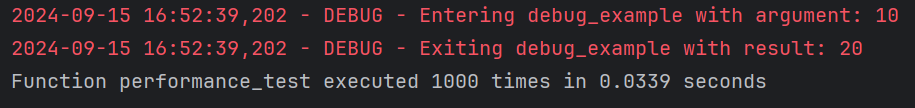
\includegraphics[width=0.5\linewidth]{学习6.png}
  % 图片标题
  \captionof{figure}{timeit计算运行时间}
  \label{fig:example}
\end{minipage}


7.
\begin{verbatim}
     用start_time和end_time记录时间
     import time
     # 方法1:使用循环
     start_time = time.time()
     squares = []
     for i in range(1000):
       squares.append(i**2)
     end_time = time.time()
     print(f"Using loop: {end_time - start_time} seconds")       
\end{verbatim}

\noindent
\begin{minipage}{\linewidth}
 \centering
  % 插入图片
  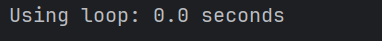
\includegraphics[width=0.5\linewidth]{学习7.png}
  % 图片标题
  \captionof{figure}{time进行时间记录}
  \label{fig:example}
\end{minipage}

8.
\begin{verbatim}
    使用memory_profiler模块来分析函数内存使用情况
    from memory_profiler import profile
    @profile
    def create_large_list():
       large_list = [0] * int(1e7)
       return large_list
    create_large_list()
\end{verbatim}

\noindent
\begin{minipage}{\linewidth}
 \centering
  % 插入图片
  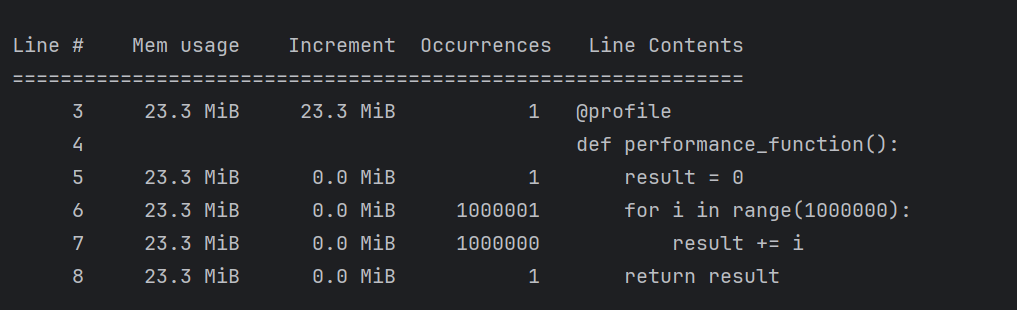
\includegraphics[width=0.5\linewidth]{学习8.png}
  % 图片标题
  \captionof{figure}{结果如图}
  \label{fig:example}
\end{minipage}

\subsection{元编程学习例子9个}

1. 使用装饰器修饰函数
\begin{verbatim}
    def debug(func):
    def wrapper(*args, **kwargs):
       print(f"Calling function: {func.__name__}")
       result = func(*args, **kwargs)
       print(f"Function {func.__name__} returned: {result}")
       return result
    return wrapper
    @debug
    def add(a, b):
       return a + b
    # 调用装饰过的函数
    add(3, 4)
\end{verbatim}

\begin{minipage}{\linewidth}
    \centering
     % 插入图片
     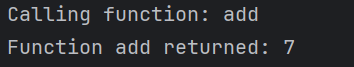
\includegraphics[width=0.5\linewidth]{学习9.png}
     % 图片标题
     \captionof{figure}{调用装饰过函数后的结果}
     \label{fig:example}
\end{minipage}


2.使用装饰器修饰类
\begin{verbatim}
    def add_property(cls):
      cls.new_property = "This is a new property"
      return cls
    @add_property
    class MyClass:
     pass
    # 检查新属性
    print(MyClass.new_property)
\end{verbatim}


\noindent
\begin{minipage}{\linewidth}
 \centering
  % 插入图片
  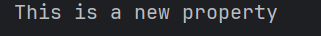
\includegraphics[width=0.5\linewidth]{学习10.png}
  % 图片标题
  \captionof{figure}{调用装饰过类后的结果}
  \label{fig:example}
\end{minipage}




3.
\begin{verbatim}
    动态属性访问: 使用__getattr__和__setattr__可以拦截对属性的访问和赋值。
    由于__getattr__魔术方法的存在,即使name和age在DynamicAttributes类中没有定义,
    这些属性也会从kwargs字典中获取,并正确返回。

    class DynamicAttributes:
       def __init__(self, **kwargs):
          self.kwargs = kwargs
       def __getattr__(self, attr):
          return self.kwargs.get(attr, None)
    obj = DynamicAttributes(name='John', age=30)
       print(obj.name)  # 输出: John
       print(obj.age)   # 输出: 30
\end{verbatim}


\noindent
\begin{minipage}{\linewidth}
  \centering
  % 插入图片
  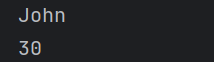
\includegraphics[width=0.5\linewidth]{学习11.png}
  % 图片标题
  \captionof{figure}{元编程动态属性访问}
  \label{fig:example}
\end{minipage}

4.
\begin{verbatim} 
    使用Python的内置函数type来动态创建一个类
    def create_class(name, bases, attrs):
       return type(name, bases, attrs)
    MyClass = create_class('MyClass', (object,), {'x': 5})
    print(MyClass)
    print(MyClass.x)
\end{verbatim}

\noindent
\begin{minipage}{\linewidth}
  \centering
  % 插入图片
  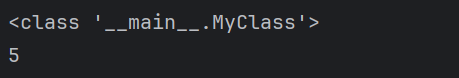
\includegraphics[width=0.5\linewidth]{学习12.png}
  % 图片标题
  \captionof{figure}{用type动态创建一个类}
  \label{fig:example}
\end{minipage}

5.使用修饰器改变函数行为
\begin{verbatim}
    from functools import wraps
    def add_hello(func):
        @wraps(func)
        def wrapper(*args, **kwargs):
           print("Hello")
           return func(*args, **kwargs)
        return wrapper
     @add_hello
    def say_goodbye():
           print("Goodbye")
    say_goodbye()
\end{verbatim}

\noindent
\begin{minipage}{\linewidth}
 \centering
  % 插入图片
  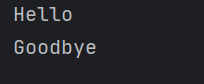
\includegraphics[width=0.5\linewidth]{学习13.png}
  % 图片标题
  \captionof{figure}{使用修饰器改变函数行为}
  \label{fig:example}
\end{minipage}



6.使用exec函数动态执行了一段包含函数定义的字符串代码,
然后调用这个新定义的函数,并输出结果

\begin{verbatim}
    code = "def hello(): print('Hello World')"
    exec(code)
    hello()  # 输出: Hello World
\end{verbatim}


\noindent
\begin{minipage}{\linewidth}
 \centering
  % 插入图片
  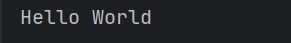
\includegraphics[width=0.5\linewidth]{学习14.png}
  % 图片标题
  \captionof{figure}{hello()输出后的结果}
  \label{fig:example}
\end{minipage}

7.\begin{verbatim}
    用functools.partial创建部分函数应用
    from functools import partial
    def multiply(x, y):
         return x * y
    double = partial(multiply, 2)
    print(double(3))  # 输出: 6
  \end{verbatim}

\noindent
\begin{minipage}{\linewidth}
 \centering
  % 插入图片
  
\includegraphics[width=0.5\linewidth]{学习15.png}
  % 图片标题
  \captionof{figure}{用functools.partial创建部分函数应用}
  \label{fig:example}
\end{minipage}

8.
\begin{verbatim}
    class MyCallable:
    def __init__(self, value):
        self.value = value
    def __call__(self):
        print(self.value)
    callable_obj = MyCallable("Hello")
    callable_obj()  # 输出: Hello
\end{verbatim}

\noindent
\begin{minipage}{\linewidth}
 \centering
  % 插入图片
  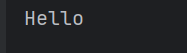
\includegraphics[width=0.5\linewidth]{学习16.png}
  % 图片标题
  \captionof{figure}{输出结果:}
  \label{fig:example}
\end{minipage}

9.
\begin{verbatim}
   使用__slots__限制对象属性
   class MyClass:
       __slots__ = ['name']
   def __init__(self, name):
       self.name = name
   obj = MyClass('John')
   obj.age = 30  
   print(obj.name)  # 输出: John
   print(obj.age)   # 输出: AttributeError: 'MyClass' object has no attribute 'age'
\end{verbatim}

\noindent
\begin{minipage}{\linewidth}
 \centering
  % 插入图片
  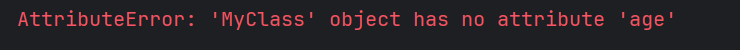
\includegraphics[width=0.5\linewidth]{学习17.png}
  % 图片标题
  \captionof{figure}{限制对象属性输出结果}
  \label{fig:example}
\end{minipage}


\subsection{Pytorch简单学习例子3个}
1.张量的使用 
\begin{verbatim}
     import torch
     # 创建一个张量
     a = torch.tensor([1, 2, 3])
     print(a)
     # 加法操作
     b = torch.tensor([4, 5, 6])
     sum_ab = a + b
     print(sum_ab)
     # 乘法操作
     product_ab = a * b
     print(product_ab)
\end{verbatim}


\begin{minipage}{\linewidth}
    \centering
     % 插入图片
     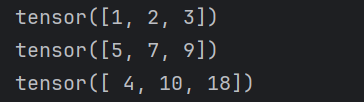
\includegraphics[width=0.5\linewidth]{学习18.png}
     % 图片标题
     \captionof{figure}{张量的使用}
     \label{fig:example}
\end{minipage}



2.用Pytorch对值进行预测
\begin{verbatim}
        import torch
        import torch.nn as nn
        import torch.optim as optim
        # 定义一个简单的线性回归模型
        class LinearRegressionModel(nn.Module):
            def __init__(self, input_dim, output_dim):
                super(LinearRegressionModel, self).__init__()
                # 定义一个线性层,即矩阵乘法层
                self.linear = nn.Linear(input_dim, output_dim)

            def forward(self, x):
                # 应用线性层,即执行矩阵乘法
                out = self.linear(x)
                return out
        # 设置输入和输出的维度
        input_dim = 1  # 假设我们只有一个特征
        output_dim = 1  # 假设我们预测一个值
        # 实例化模型
        model = LinearRegressionModel(input_dim, output_dim)
        # 定义损失函数和优化器
        criterion = nn.MSELoss()  # 均方误差损失函数
        optimizer = optim.SGD(model.parameters(), lr=0.01)  # 随机梯度下降优化器
        # 生成一些随机数据来模拟训练过程
        # 假设我们的数据集是 y = 2x + 1
        x_train = torch.randn(100, input_dim)  # 100个样本,每个样本一个特征
        y_train = 2 * x_train + 1  # 真实值
        # 训练模型
        num_epochs = 1000  # 训练的轮数
        for epoch in range(num_epochs):
            # 前向传播
            outputs = model(x_train)

            # 计算损失
            loss = criterion(outputs, y_train)

            # 清零梯度
            optimizer.zero_grad()

            # 反向传播和优化
            loss.backward()
            optimizer.step()

            if (epoch + 1) % 100 == 0:
                print(f'Epoch [{epoch + 1}/{num_epochs}], Loss: {loss.item():.4f}')

        # 测试模型
        with torch.no_grad():  # 在这个上下文中,不需要计算梯度
            predicted = model(x_train).data.numpy()  # 获得预测值
            actual = y_train.data.numpy()  # 获得真实值
            print(f'Predicted: {predicted[:5]}')
            print(f'Actual: {actual[:5]}')

\end{verbatim}



\noindent
\begin{minipage}{\linewidth}
 \centering
  % 插入图片
  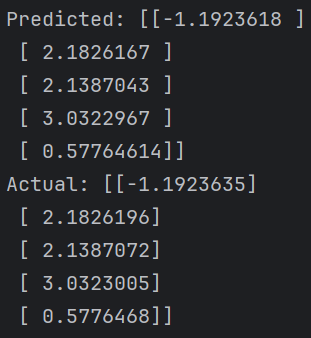
\includegraphics[width=0.5\linewidth]{学习19.png}
  % 图片标题
  \captionof{figure}{预测和真实结果}
  \label{fig:example}
\end{minipage}


3.用Pytorch建立网络
\begin{verbatim}
    import torch.nn as nn
    import torch.nn.functional as F

    # 定义一个网络
    class Net(nn.Module):

        def __init__(self):
            super(Net, self).__init__()
            # 定义网络层
            self.conv1 = nn.Conv2d(1, 6, 3)  # 输入通道1,输出通道6,3x3卷积核
            self.conv2 = nn.Conv2d(6, 16, 3)
            # 定义全连接层
            self.fc1 = nn.Linear(16 * 6 * 6, 120)  # 6*6从图像维度推断
            self.fc2 = nn.Linear(120, 84)
            self.fc3 = nn.Linear(84, 10)

        def forward(self, x):
            # 在网络前向传播过程中定义数据流
            x = F.max_pool2d(F.relu(self.conv1(x)), (2, 2))
            x = F.max_pool2d(F.relu(self.conv2(x)), 2)
            x = x.view(-1, self.num_flat_features(x))
            x = F.relu(self.fc1(x))
            x = F.relu(self.fc2(x))
            x = self.fc3(x)
            return x

        def num_flat_features(self, x):
            size = x.size()[1:]  # 除去批处理维度的其他所有维度
            num_features = 1
            for s in size:
                num_features *= s
            return num_features

    net = Net()
    print(net)

\end{verbatim}


\noindent
\begin{minipage}{\linewidth}
 \centering
  % 插入图片
  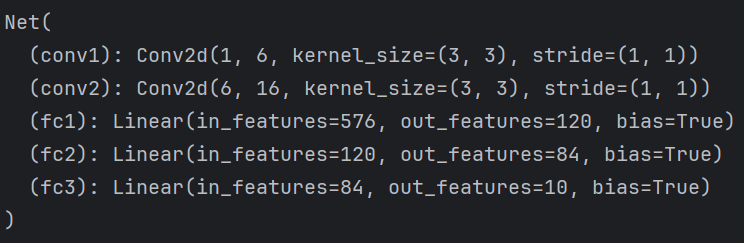
\includegraphics[width=0.5\linewidth]{学习20.png}
  % 图片标题
  \captionof{figure}{网络建立后的结果}
  \label{fig:example}
\end{minipage}




\section{解题感悟}
代码调试和性能分析让我有条不紊地解决代码的问题
调试让我学会了耐心和细致,
而性能分析则教会了我如何追求效率与实用。
这些技能提升了我的编程能力,也使我明白了持续优化和创新的重要性。

元编程让我意识到,代码不仅仅是静态的指令集合,而是一种可以动态变化、自我进化的实体。
在学习元编程的过程中,我感受到了元编程的高效与灵活。
但是元编程带来的灵活性和抽象性也可能会让代码变得难以理解和维护,因此在使用时需要谨慎和节制。

学习PyTorch,则是我进入深度学习领域的开始。PyTorch的直观性和易用性让我迅速上手,它的动态计算图让我能够轻松地构建和调试复杂的神经网络。
在这个过程中,我感受到了深度学习的强大。

总的来说,学习元编程和PyTorch编程让我感受到了编程的深度和广度,它们不仅提升了我的技术能力,也激发了我对技术和创新的热爱。
在这个过程中,我学会了如何更好地利用工具,如何面对复杂问题,以及如何在不断变化的技术领域中保持学习和成长。

github路径
您可以在此查看项目的源代码: 

\url{https://github.com/AmbitiousLight/AmbitiousLight/tree/cd6bbe282633d03ad085f0014ba46766355632b4/shell%E5%92%8Cvim}

\end{document}
